%%%%%%%%%%%%%%%%%%%%%%%%%%%% BEGIN PROGRAMMING MODEL %%%%%%%%%%%%%%%%%%%%%%%%%%%

The imagination-based planning (IBP) for reinforcement learning framework~\cite{PascanuetalCoRR-17} serves as an example for how the code synthesis module might be implemented. The IBP architecture combines three separate adaptive components: (a) the {\it{controller}} + {\it{memory}} system which maps a state $s \in S$ and history $h \in H$ to an action $a \in A$; (b) the {\it{manager}} maps a history $h \in H$ to a route $u \in U$ that determines whether the system performs an action in the {\it{compute}} environment, e.g., single-step the program in the FIDE, or performs an imagination step, e.g., generates a proposal for modifying the existing code under construction; the {\it{imagination model}} is a form of dynamical systems model that maps a pair consisting of a state $s \in S$ and an action $a \in A$ to an imagined next state $s' \in S$ and scalar-valued reward $r \in R$.

The imagination model can be implemented as an interaction network~\cite{BattagliaetalNIPS-16} or using the graph-networks framework~\cite{BattagliaetalCoRR-18,SanchezetalCoRR-18}. The three components are trained by three distinct, concurrent, on-policy training loops. The IBP framework shown in Figure~{\urlh{#Graph_Nets_Imagination_Coding}{\ref{fig_imagine}}} allows code synthesis to alternate between exploiting by modifying and running code, and exploring by using the model to investigate and analyze what would happen if you actually did act. The manager chooses whether to execute a command or predict (imagine) its result and can generate any number of trajectories to produce a tree $h_t$ of imagined results. The controller takes this tree plus the compiled history and chooses an action (command) to carry out in the FIDE.

%%% %%%%%%%%%%%%%%%%%%%%%%%%%%%%%%%%%%%%%%%%%%%%%%%%%%%%%%%%%%%%%%%%%%%%%%%%%%%%

%%% Figure~{\urlh{#Graph_Nets_Imagination_Coding}{\ref{fig_imagine}}}
\begin{figure}
%
  \begin{center} 
%    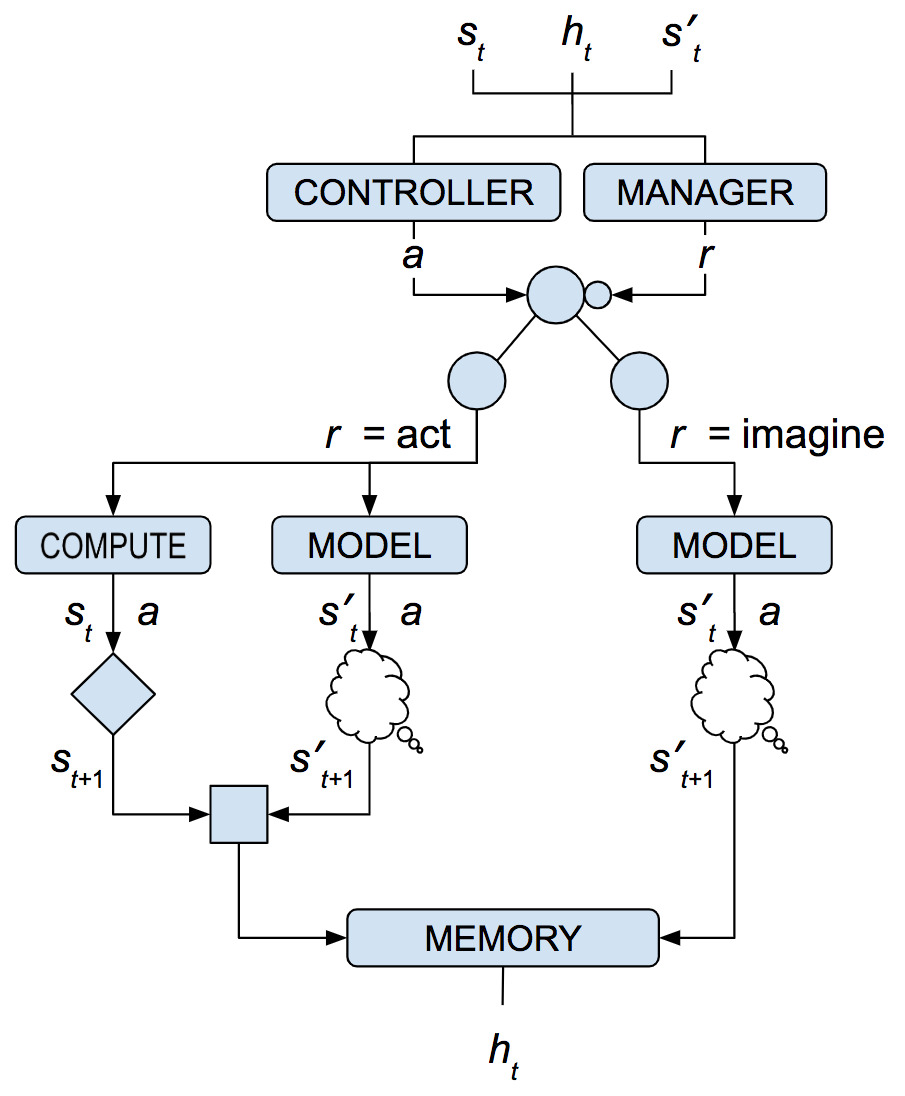
\includegraphics[width=4.3125in]{./figures/Graph_Nets_Imagination_Coding.png} % 905 × 1096 pixels
    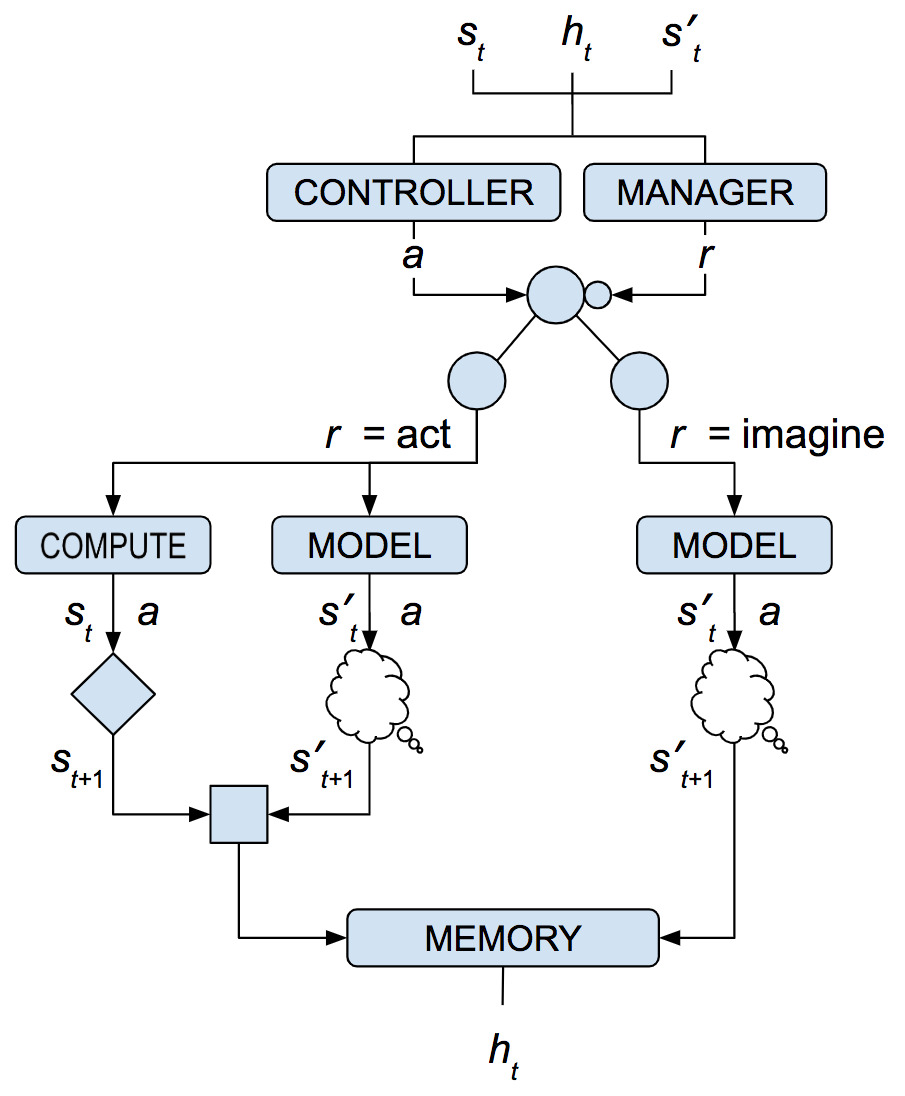
\includegraphics[width=2.15in]{./figures/Graph_Nets_Imagination_Coding.png} % 905 × 1096 pixels
  \end{center}
%
  \caption{The above graphic illustrates how we might adapt the imagination-based planning (IBP) for reinforcement learning framework~\cite{PascanuetalCoRR-17} for use as the core of the apprentice code synthesis module. Actions in this case correspond to transformations of the program under development. States incorporate the history of the evolving partial program. Imagination consists of exploring sequences of program transformations.}
%
  \label{fig_imagine}
%
\end{figure}

%%%%%%%%%%%%%%%%%%%%%%%%%%%%%% END PROGRAMMING MODEL %%%%%%%%%%%%%%%%%%%%%%%%%%%
